% GNUPLOT: LaTeX picture with Postscript
\begingroup
  \makeatletter
  \providecommand\color[2][]{%
    \GenericError{(gnuplot) \space\space\space\@spaces}{%
      Package color not loaded in conjunction with
      terminal option `colourtext'%
    }{See the gnuplot documentation for explanation.%
    }{Either use 'blacktext' in gnuplot or load the package
      color.sty in LaTeX.}%
    \renewcommand\color[2][]{}%
  }%
  \providecommand\includegraphics[2][]{%
    \GenericError{(gnuplot) \space\space\space\@spaces}{%
      Package graphicx or graphics not loaded%
    }{See the gnuplot documentation for explanation.%
    }{The gnuplot epslatex terminal needs graphicx.sty or graphics.sty.}%
    \renewcommand\includegraphics[2][]{}%
  }%
  \providecommand\rotatebox[2]{#2}%
  \@ifundefined{ifGPcolor}{%
    \newif\ifGPcolor
    \GPcolortrue
  }{}%
  \@ifundefined{ifGPblacktext}{%
    \newif\ifGPblacktext
    \GPblacktexttrue
  }{}%
  % define a \g@addto@macro without @ in the name:
  \let\gplgaddtomacro\g@addto@macro
  % define empty templates for all commands taking text:
  \gdef\gplbacktext{}%
  \gdef\gplfronttext{}%
  \makeatother
  \ifGPblacktext
    % no textcolor at all
    \def\colorrgb#1{}%
    \def\colorgray#1{}%
  \else
    % gray or color?
    \ifGPcolor
      \def\colorrgb#1{\color[rgb]{#1}}%
      \def\colorgray#1{\color[gray]{#1}}%
      \expandafter\def\csname LTw\endcsname{\color{white}}%
      \expandafter\def\csname LTb\endcsname{\color{black}}%
      \expandafter\def\csname LTa\endcsname{\color{black}}%
      \expandafter\def\csname LT0\endcsname{\color[rgb]{1,0,0}}%
      \expandafter\def\csname LT1\endcsname{\color[rgb]{0,1,0}}%
      \expandafter\def\csname LT2\endcsname{\color[rgb]{0,0,1}}%
      \expandafter\def\csname LT3\endcsname{\color[rgb]{1,0,1}}%
      \expandafter\def\csname LT4\endcsname{\color[rgb]{0,1,1}}%
      \expandafter\def\csname LT5\endcsname{\color[rgb]{1,1,0}}%
      \expandafter\def\csname LT6\endcsname{\color[rgb]{0,0,0}}%
      \expandafter\def\csname LT7\endcsname{\color[rgb]{1,0.3,0}}%
      \expandafter\def\csname LT8\endcsname{\color[rgb]{0.5,0.5,0.5}}%
    \else
      % gray
      \def\colorrgb#1{\color{black}}%
      \def\colorgray#1{\color[gray]{#1}}%
      \expandafter\def\csname LTw\endcsname{\color{white}}%
      \expandafter\def\csname LTb\endcsname{\color{black}}%
      \expandafter\def\csname LTa\endcsname{\color{black}}%
      \expandafter\def\csname LT0\endcsname{\color{black}}%
      \expandafter\def\csname LT1\endcsname{\color{black}}%
      \expandafter\def\csname LT2\endcsname{\color{black}}%
      \expandafter\def\csname LT3\endcsname{\color{black}}%
      \expandafter\def\csname LT4\endcsname{\color{black}}%
      \expandafter\def\csname LT5\endcsname{\color{black}}%
      \expandafter\def\csname LT6\endcsname{\color{black}}%
      \expandafter\def\csname LT7\endcsname{\color{black}}%
      \expandafter\def\csname LT8\endcsname{\color{black}}%
    \fi
  \fi
    \setlength{\unitlength}{0.0500bp}%
    \ifx\gptboxheight\undefined%
      \newlength{\gptboxheight}%
      \newlength{\gptboxwidth}%
      \newsavebox{\gptboxtext}%
    \fi%
    \setlength{\fboxrule}{0.5pt}%
    \setlength{\fboxsep}{1pt}%
\begin{picture}(14400.00,3600.00)%
    \gplgaddtomacro\gplbacktext{%
      \csname LTb\endcsname%%
      \put(1210,1459){\makebox(0,0)[r]{\strut{}$0.0001$}}%
      \put(1210,1746){\makebox(0,0)[r]{\strut{}$0.001$}}%
      \put(1210,2033){\makebox(0,0)[r]{\strut{}$0.01$}}%
      \put(1210,2321){\makebox(0,0)[r]{\strut{}$0.1$}}%
      \put(1210,2608){\makebox(0,0)[r]{\strut{}$1$}}%
      \put(1210,2895){\makebox(0,0)[r]{\strut{}$10$}}%
      \put(1608,1327){\rotatebox{-28}{\makebox(0,0)[l]{\strut{}\normalCache($ \cachesetNmbr\!=\!1$)}}}%
      \put(2141,1327){\rotatebox{-28}{\makebox(0,0)[l]{\strut{}\normalCache($ \cachesetNmbr\!=\!2$)}}}%
      \put(2674,1327){\rotatebox{-28}{\makebox(0,0)[l]{\strut{}\normalCache($ \cachesetNmbr\!=\!4$)}}}%
      \put(3207,1327){\rotatebox{-28}{\makebox(0,0)[l]{\strut{}\normalCache($ \cachesetNmbr\!=\!8$)}}}%
      \put(3740,1327){\rotatebox{-28}{\makebox(0,0)[l]{\strut{}\normalCache($\cachesetNmbr\!=\!16$)}}}%
      \put(4273,1327){\rotatebox{-28}{\makebox(0,0)[l]{\strut{}\scatterCacheAbbr($ \cachesetNmbr\!=\!1$)}}}%
      \put(4806,1327){\rotatebox{-28}{\makebox(0,0)[l]{\strut{}\scatterCacheAbbr($ \cachesetNmbr\!=\!2$)}}}%
      \put(5339,1327){\rotatebox{-28}{\makebox(0,0)[l]{\strut{}\scatterCacheAbbr($ \cachesetNmbr\!=\!4$)}}}%
      \put(5872,1327){\rotatebox{-28}{\makebox(0,0)[l]{\strut{}\scatterCacheAbbr($ \cachesetNmbr\!=\!8$)}}}%
      \put(6405,1327){\rotatebox{-28}{\makebox(0,0)[l]{\strut{}\scatterCacheAbbr($\cachesetNmbr\!=\!16$)}}}%
      \put(6938,1327){\rotatebox{-28}{\makebox(0,0)[l]{\strut{}\phantomCacheAbbr($ \cachesetNmbr\!=\!1,\phantomR\!=\!1$)}}}%
      \put(7471,1327){\rotatebox{-28}{\makebox(0,0)[l]{\strut{}\phantomCacheAbbr($ \cachesetNmbr\!=\!4,\phantomR\!=\!1$)}}}%
      \put(8004,1327){\rotatebox{-28}{\makebox(0,0)[l]{\strut{}\phantomCacheAbbr($ \cachesetNmbr\!=\!8,\phantomR\!=\!1$)}}}%
      \put(8537,1327){\rotatebox{-28}{\makebox(0,0)[l]{\strut{}\phantomCacheAbbr($ \cachesetNmbr\!=\!16,\phantomR\!=\!2$)}}}%
      \put(9070,1327){\rotatebox{-28}{\makebox(0,0)[l]{\strut{}\phantomCacheAbbr($ \cachesetNmbr\!=\!4,\phantomR\!=\!2$)}}}%
      \put(9603,1327){\rotatebox{-28}{\makebox(0,0)[l]{\strut{}\phantomCacheAbbr($ \cachesetNmbr\!=\!8,\phantomR\!=\!2$)}}}%
      \put(10136,1327){\rotatebox{-28}{\makebox(0,0)[l]{\strut{}ShortSpec}}}%
      \put(10510,1327){\rotatebox{-28}{\makebox(0,0)[l]{\strut{}ShortSpec+\declassify{}}}}%
      \put(10883,1327){\rotatebox{-28}{\makebox(0,0)[l]{\strut{}LongSpec}}}%
      \put(11256,1327){\rotatebox{-28}{\makebox(0,0)[l]{\strut{}LongSpec+\declassify{}}}}%
      \put(11629,1327){\rotatebox{-28}{\makebox(0,0)[l]{\strut{}\modexp($\window\!=\!1$)}}}%
      \put(12002,1327){\rotatebox{-28}{\makebox(0,0)[l]{\strut{}\modexp($\window\!=\!2$)}}}%
      \put(12375,1327){\rotatebox{-28}{\makebox(0,0)[l]{\strut{}\modexp($\window\!=\!4$)}}}%
      \put(12748,1327){\rotatebox{-28}{\makebox(0,0)[l]{\strut{}\modexp($\window\!=\!6$)}}}%
      \put(13121,1327){\rotatebox{-28}{\makebox(0,0)[l]{\strut{}\modexp($\window\!=\!8$)}}}%
    }%
    \gplgaddtomacro\gplfronttext{%
      \csname LTb\endcsname%%
      \put(341,2177){\rotatebox{-270}{\makebox(0,0){\strut{}Time for one estimation (s)}}}%
      \csname LTb\endcsname%%
      \put(1933,3416){\makebox(0,0)[l]{\strut{}Unshared-\interferenceSetSamples}}%
      \csname LTb\endcsname%%
      \put(1933,3174){\makebox(0,0)[l]{\strut{}Shared-\interferenceSetSamples}}%
      \csname LTb\endcsname%%
      \put(5824,3416){\makebox(0,0)[l]{\strut{}Shared($\forall \blockIdx: \ACIFn{}(\loadVar)[\blockIdx]=0$)-\interferenceSetSamples}}%
      \csname LTb\endcsname%%
      \put(5824,3174){\makebox(0,0)[l]{\strut{}Unshared-\noninterferenceSetSamples}}%
      \csname LTb\endcsname%%
      \put(9715,3416){\makebox(0,0)[l]{\strut{}Shared-\noninterferenceSetSamples}}%
      \csname LTb\endcsname%%
      \put(9715,3174){\makebox(0,0)[l]{\strut{}Shared($\forall \blockIdx: \ACIFn{}(\loadVar)[\blockIdx]=0$)-\noninterferenceSetSamples}}%
    }%
    \gplbacktext
    \put(0,0){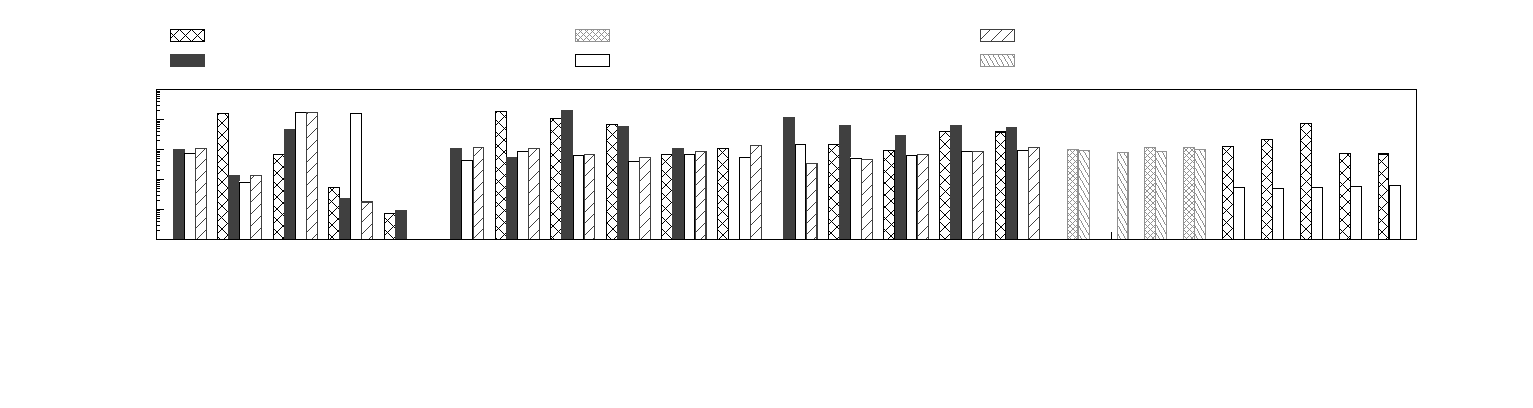
\includegraphics[width={720.00bp},height={180.00bp}]{sampletime}}%
    \gplfronttext
  \end{picture}%
\endgroup
